%   Dans l'introduction, on présente le problème étudié et les buts
% poursuivis. L'introduction permet de faire connaître le cadre de la
% recherche et d'en préciser le domaine d'application. Elle fournit
% les précisions nécessaires en ce qui concerne le contexte de
% réalisation de la recherche, l'approche envisagée, l'évolution de
% la réalisation. En fait, l'introduction présente au lecteur ce
% qu'il doit savoir pour comprendre la recherche et en connaître la
% portée.
\Chapter{INTRODUCTION}\label{sec:Introduction}  
Altough Linux uses Git as its version control system, most developer cannot commit directly to the repository. In fact, the developers and maintainers use several different repositories in the development process. The main repository (also called the main tree, of the main line) is maintained by Linus Torvald, the creator of Linux. For a developer to have their code changes integrated into an official release of the Linux Kernel, their changes must be submitted and accepted by Linus Torvalds, as he has the last word on any code being added to the main tree. 

Submitting code changes \textit{upstream}, means to submit changes hoping they will be \textit{merged} into the main tree, and thus into an official Linux release. To achieve this, there is a set of guidelines to follow, as the Linux Kernel follows a strict development cadence and has high code quality standards. First, the code submitted must follow the Linux coding style \footnote{\url{https://01.org/linuxgraphics/gfx-docs/drm/process/coding-style.html}}. It is important to impose a strict coding style in projects of the scale of the linux kernel. Code comming from tens of thousands of developers would become very hard to maintain is everyone cubmitted code with their own coding style. 

Secondly, developers must follow the submission process guidelines. In the vast majority of cases, developers submit their changes to a maintainer. A maintainer is in charge of maintaining a specifi subsystem. A subsystem can be represented as a series of files that work together to serve a certain purpose. When a developer is unsure of who to send the changes to, they can consult the \texttt{MAINTAINERS} file, or use the script \texttt{get\_maintainer.pl} to discover persone responsible for a certain file. The developer must send her changes in the form of a patch the modified subsystem's mailing list. 

Naturally, maintainers must review the patches to ensure that they are worthy of being integrated into their subsytem tree. These reviews usally occur in the email thread following the email patch. The patch author will probably have to improve their code changes according to the maintainer's reviews. If maintainers are satisfied with a patch, they will \textit{commit} it to their repository. As explained in \autoref{sec:commit_anatomy}, for each commit, git differenciates between the \textbf{commit author} and the \textbf{commit committer}. 

Before submitting changes to Linus, maintainers usually send the changes acquired in their repository to \textit{linux-next}\footnote{\url{https://01.org/linuxgraphics/gfx-docs/drm/process/howto.html\#becoming-a-kernel-developer}}. They may do so through an email as a patch, although submitting large changes is easier throught Git. Linux-next is where the integration testing occurs. This is where developers and maintainers make sure new code changes do not interfere with the rest of the code base and do not introduce any bugs. Linus will pull commits that have been in the -next tree for a few weeks \footnote{\url{https://01.org/linuxgraphics/gfx-docs/drm/process/howto.html\#becoming-a-kernel-developer}}. Linux-next ensures important bugs introduced by new commits are discovered and dealt with before being committed to the main tree, as these bugs would drastically slow down the release cycle. 


The main tree uses a specific releace cycle. After a new version is released, 4.13 for instance, the \textit{merge window} opens for release 4.14. This two-week long merge window is the only opportunity to submit new code changes in hope to have them integrated in release 4.14. Linus pulls most of the changes from linux-next during that time period because these changes are les likely to cause bugs and thus delay the next release. After two weeks, the merge window closes and linux 4.14-rc1 is released. Then, developers work on ensuring that the kernel is as stable as possible. For approximately 6 to 8 weeks, linus will only accept patches that address bugs introduced by commits merged during the merge window. The only exception is new drivers. New drivers can be submitted outside of the merge window because bugs introduced by drivers are self contained, and only affect users using the specific driver. A new -rc comes out about every week, until Linus declares that the kernel is stable enough to be released. 

Furthermore, large subsytems impose their own release schedule to developers. For instance, the Net subsystem also has two main trees: \texttt{net} and \texttt{net-next}. Net-next recieves all changes submitted to the net subsystem. Once the linus' merge window opens, net-next closes, and all the changes accumulated over the last 10 weeks will be submitted to the main tree. At this point, the net tree will recieve all the fixed related to commits that were committed to the main tree. Once Linus' merge window closes, net-next reopens and developers are free to submit new patches again. 

As stated above, the contribution process relies heavily on emails. The reason why the linux community does not use tools such as github or gerrit is that those tools would not scale to the size of the linux community \citep{armstrong}. And even though the email-based system has been very reliable over the lifetime of the project, there is one drawback. Once a patch is committed to the subsytem tree, and after the commit makes its way upstream to the main tree, there is no easy way to recover the review discussions that took place in the mailing list. 

The process described above shows the number of different activities in which Linux developers participate. In particular, maintainers, who are regarded as experts by the rest of the community, tend to participate in a larger array of activities than other developers. In fact, Maintainers are often the only people allowed to commit to the subsystem's git repository. Their role being crucial to their subsystem, it is important to be able to find a replacement for them if they decided to give up their maintainer responsibilities.

% \footnote{\url{https://01.org/linuxgraphics/gfx-docs/drm/process/howto.html#becoming-a-kernel-developer}}
% \footnote{\url{https://www.kernel.org/doc/Documentation/networking/netdev-FAQ.txt}}

% linux pulling from linux next: https://www.kernel.org/doc/man-pages/linux-next.html

% linux stable: https://01.org/linuxgraphics/gfx-docs/drm/process/howto.html#x-y-stable-kernel-tree






% original intro

Employee turn over represents a risk for software organizations. \citep{turnover} claim that the cost associated to replacing a developer can be up to 1.5 times the developer's salary. As an answer to this risks in software engineering organizations, researchers have attempted to establish models capable of finding experts in certain code areas. By recommending experienced developers, these models would ease the difficulty of replacing current experts as they leave the organization. 


Introduced in the early 2000s\citep{mockus02}\citep{McDonald}, these models were using the developers' coding activities to assess their expertise. Their activity was quantified in terms of two simple metrics: number of \ac{LOC} and number of commits, which represents the amount of change brought to the source code. 

The Linux Kernel, for instance, is a 26-year-old project that has experienced a drastic growth in terms of code base and in terms of developer community. Wanting to keep a high standard of code quality and a fast release system, the community had to implement a hierarchical contribution system. In this contribution system, some developers are responsible for the maintenance of their subsystems. These developers, or maintainers, are trusted by the rest of the Linux community to be skilled enough to ensure the durability of their subsystem. This trust was acquired by contributing to the subsystem over the years. However, when trying to use traditional expertise determining metrics in the linux kernel, maintainers are rarely recomended. Our results indicate that the number of lines of code only correctly assess less than 50\% of experts and number of commits authored only finds 25\% of experts. 


We believe that previous expertise models fail to take into account some critical aspect of large scale software development. As subsystems become larger and welcome more contributors, maintainers have to dedicate more of their time reviewing other developers' contributions to maintain code quality. Our results indicate that this shift towards a managerial position is usually followed by a drop in code contributions by that person. This implies that, in the eye of a model looking at only \ac{LOC} and commits, the maintainer will lose expertise. 

Additionally, previous models do not take into account the amount of time a developer has been involved in the development of the project. Measuring previous contributions could help quantifying a developer's experience and the expertise she acquired over the years. 

We introduce a new expertise model adapted to large software organizations like the Linux community. Our model is better suited for the Linux community because it can take into account all the activities undertaken by both maintainers and developers. In addition to quantifying different activities, we use add a historical percpective to the model to take into account the previous contributions made by the developers. This thesis provides an in-depth description of the different steps necessary for the creation of this model as well as an evaluation of the accuracy of our model. 



\section{Hypothesis of Thesis}

Our main research objective is to create a model capable of detecting experts in a certain code area. \autoref{sec:expertise_models} describes previous expertise models created over the years. Our evalution, provided in chapter5, indicates that previous models are not well suited for the linux community. Thus, We based our model on a series of new metrics, which were acquired through different techniques. We were able to make some of these metrics available to the community through two open source projects, which are described in Chapter 3.


\textbf{Hypothesis:} Expertise models targeting large software engineering organizations require a look at all development activities, including code reviews and upstream committing.



To explore this hypothesis, we evaluate the relevance of the different activities present in large scale software development for the purpose of measuring expertise. We build an expertise model based on metrics quantifying these activities. Moreover, we include a hirtorical dimention to the model to represent the impact of long term involvement with the software project. Finally, we provide an evaluation of the different activities by comparing the expert recommendations to the data listed in the \texttt{MAINTAINERS} file.

We build an expertise model which considers a widder aray of metric to assess developer expertise. Since the Linux contribution process is similar to the one used by other organizations, this model could be accurate in other large software projects. 




\section{Plan of the Thesis}


The structure of this thesis is as follows. We conduct a litterature review in chapter 2, where we describe previous expertise models and other topics of interest. Chapter 3 gives a detailed overview of the general workflow of the thesis. Chapter 4 gives an indepth look at Email2git, one of the opensourcve project we created. Finally, chapter 5 includes the article we submitted to the  International Conference on Software Analysis, Evolution and Reengineering (SANER).



% Un URL: \href{http://www.polymtl.ca}{École Polytechnique de Montréal}.

% \subsubsection{Une sous-sous-section}
% Les besoins des flots de données peuvent être catégorisés selon
% quatre paramètres importants \citep[voir][sect.\,5.4]{Tanenbaum} ou:
% \begin{itemize}
% %%
% %% ELEMENTS DE LA PROBLEMATIQUE
% %%
% \section{Éléments de la problématique}  % environ 3 pages
% La description de \mbox{l'en-tête} commun de RSVP est détaillée ci-dessous:\\
% \begin{tabular}{p{1in}p{4.5in}}
% &\\ % Ligne vide
% \texttt{Ver}: & \texttt{4 bits}\\
%           & Version du protocole. La version actuelle est~1.\\[5pt]
% \texttt{Flags}: & \texttt{4 bits}\\
%           & Aucun Flag n'est défini. L'émetteur doit (\textbf{MUST})
%           mettre le champ à zéro et le récepteur doit (\textbf{MUST})
%           ignorer ce champ.\\[5pt]
% \texttt{Msg Type}: & \texttt{8 bits}\\
%           & Type de message\\[5pt]
% \texttt{Checksum}: & \texttt{16 bits}\\
%           & Complément à un du complément à un de la somme des champs
%           de \mbox{l'en-tête}, avec le champ Checksum à~0 pour des
%           fins de calcul. La valeur~0 signifie qu'aucun Checksum n'a
%           été transmis. Si le résultat du calcul du Checksum donne~0,
%           la valeur 0xFFFF doit être stockée dans ce champ.\\[5pt]
% \texttt{TTL}: & \texttt{8 bits}\\
%           & Valeur originelle du champ \texttt{TTL} utilisée pour
%           transmettre ce message.\\[5pt]
% \texttt{Reserved}: & \texttt{8 bits}\\
%           & Réservé pour usage futur. L'émetteur doit (\textbf{MUST})
%           mettre le champ à zéro et le récepteur doit (\textbf{MUST})
%           ignorer ce champ.\\[5pt]
% \texttt{Length}: & \texttt{16 bits}\\
%           & Longueur totale du message en octets, incluant
%           \mbox{l'en-tête} commun et tous les objets de longueur
%           variable.
% \end{tabular}

% \subsection{Autres types de structures de données}
% L'énumération:
% \begin{enumerate}
% \item Un item~;
% \item Un autre item.
% \end{enumerate}


% \subsection{Le protocole IPv6}
% Voir la Figure~\ref{fig:IPv6} pour plus de détails. Le champs DSCP est
% décrit dans le Tableau~\ref{tab:RangesDSCP}.

% \begin{figure}[htb]
% \centering
% 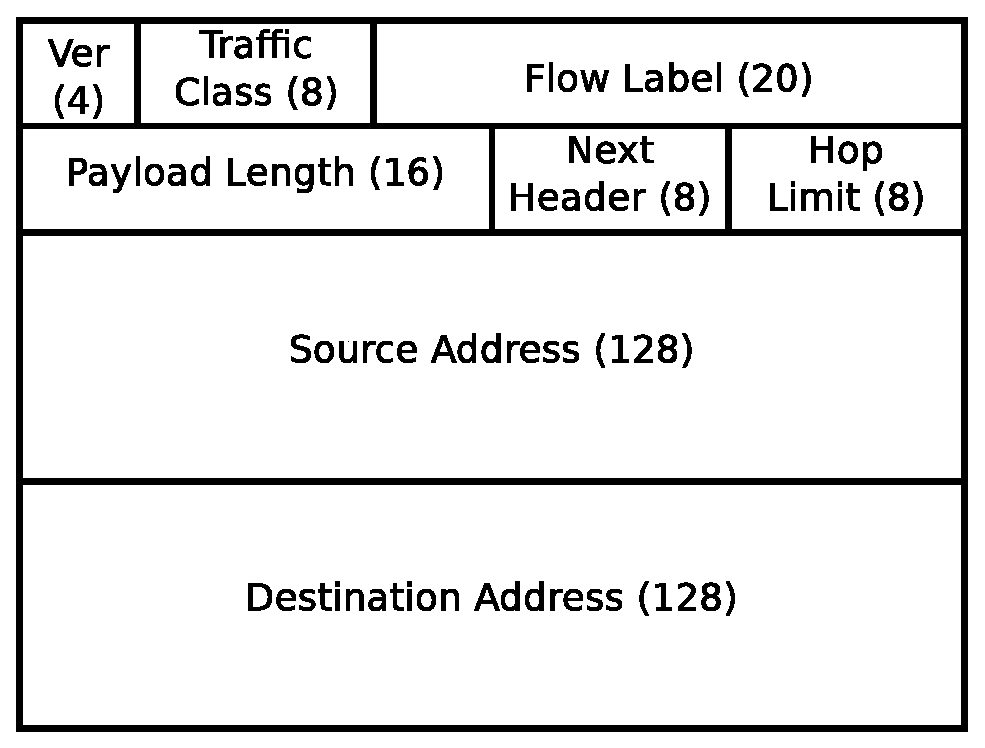
\includegraphics[width=4in]{IPv6_header}
% \caption{L'en-tête IPv6}
% \label{fig:IPv6}
% \end{figure}

% \begin{table}[ht]
% \caption{Plages de valeurs pour le champ \texttt{DSCP}}
% \centering
% \begin{tabular}{|c|c|l|}
% \hline\rowcolor[gray]{0.8}\color{black}
% Plage & Valeurs & Règle d'assignation\\\hline
% 1 & xxxxx0 & Assignation par une norme de l'IANA\\\hline
% 2 & xxxx11 & Expérimentation/Usage local\\\hline
% 3 & xxxx01 & Expérimentation/Usage local (pourrait être jointe à la plage 1)\\\hline
% \end{tabular}
% \label{tab:RangesDSCP}
% \end{table}

% % On veut éviter que la figure et le tableau soient placés au-delà de la section courante.
% \FloatBarrier


% %%
% %% OBJECTIFS DE RECHERCHE
% %%
% \section{Objectifs de recherche}  % 0.5 page
% Les objectifs de la recherche sont de concevoir un algorithme $O(n)$.


% %%
% %% PLAN DU MEMOIRE
% %%
% \section{Plan du mémoire}  % 0.5 page
% Un tableau:
% \begin{table}[htbp]
%   \centering
%   \caption{Constantes et variables du modèle analytique}
%   \begin{tabular}{|c|l|}
%     \hline\rowcolor[gray]{0.8}\color{black}
%     Symbole         & Description\\\hline
%     $\lambda$       & Taux d'arrivée moyen des requêtes de réservation de ressources\\\hline
%     $\frac{1}{\mu}$ & Durée moyenne d'une session\\\hline
%     $C$             & Capacité d'une cellule (nombre de sessions supportées)\\\hline
%     $v_{moy}$       & Vitesse moyenne des MN dans le réseau d'accès\\\hline
%     $L$             & Longueur d'un côté d'une cellule carrée\\\hline
%     $n$             & Nombre moyen de MN dans une cellule\\\hline
%     $\rho$          & Charge d'une cellule\\\hline
%     $P_b$           & Probabilité de blocage d'une requête de réservation\\\hline
%     $P_f$           & Probabilité d'interruption forcée d'une session\\\hline
%     $P_c$           & Probabilité de compléter une session avec succès\\\hline
%     $\Delta{}T$     & Délai de transmission\\\hline
%   \end{tabular}
%   \label{tab:Definitions}
% \end{table}

% La formule d'\mbox{Erlang-B}:
% \begin{equation}
%   P_b = \frac{\frac{\rho^C}{C!}}{\sum\limits_{x=0}^{C}\frac{\rho^x}{x!}}
%   \label{eq:Pblock}
% \end{equation}

% Une autre équation:
% \begin{equation}
%   \begin{split}
%     P_c &= (1 - P_b) \times (1 -  P_f)^N\\
%         &= (1 - P_b)^{N+1}
%   \end{split}
%   \label{eq:ProbComplete}
% \end{equation}

% Enfin, l'expression suivante indique le moment à partir duquel les
% réservations de ressources sont en place:
% \begin{equation}
%   \Delta{}T_{init} =
%   \begin{cases}
%     2\Delta{}T_{E2E} & \Delta{}T_{wan} > (\Delta{}T_{rad} + \Delta{}T_{net})\\
%     \Delta{}T_{E2E} + 3(\Delta{}T_{rad} + \Delta{}T_{net}) & \text{sinon}
%   \end{cases}
%   \label{eq:InitCost}
% \end{equation}

% \paragraph{Le taux de paquets perdus} correspond au nombre de paquets
% éliminés à cause d'une erreur de \emph{checksum} à un n\oe{}ud
% quelconque ou d'une situation de congestion. Le taux de paquets perdus
% pour un chemin est déterminé de la façon suivante:
% \begin{equation}
%   \label{eq:genPLR}
%   PLR_P = 1 - \prod_{i=1}^N(1 - PLR_i)
% \end{equation}

% Toutefois, si les taux d'erreurs sont très faibles, comme c'est
% généralement le cas pour des liens optiques, on peut approximer
% $PLR_P$ de façon à le transformer en un paramètre additif:
% \begin{equation}
%   \label{eq:approxPLR}
%   \begin{split}
%     PLR_{L_1 \oplus L_2} &= 1 - (1 - PLR_1)(1 - PLR_2)\\
%     &= 1 - (1 - PLR_2 - PLR_1 + \underbrace{PLR_1
%       \times PLR_2}_\text{négligeable})\qquad PLR_1 \ll 1,
%     PLR_2 \ll 1\\
%     &\approx PLR_1 + PLR_2
%   \end{split}
% \end{equation}



% Une courbe:
% \begin{figure}[htb]
% \centering
% 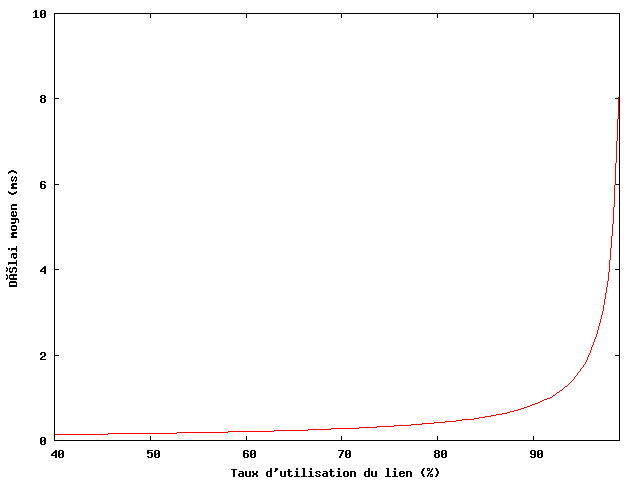
\includegraphics[width=5in]{LinkUsage}
% \caption{Délai moyen en fonction du taux d'utilisation d'un lien}
% \label{fig:LinkUse}
% \end{figure}

% \selectlanguage{english}
% This paragraph is formatted by \LaTeX{} according to the standard rules of the
% English language (\mbox{e.g.} hyphenation).
% \selectlanguage{french}

% L'arithmétique en virgule flottante peut entraîner des erreurs
% d'approximation et il est important d'en être conscient
% \citep[voir][]{Goldberg1991}.

% De même, les calculs effectués sur une carte graphique (GPU) peuvent
% introduire des erreurs d'approximation \citep{Benz2012, DSilva2012,
%   Dabrowski2011, DeDinechin2011, DeFigueiredo2004, Filliatre2007,
%   Fousse2007, Goubault2001, Goubault2008, Harder, Higham2002, Tanenbaum,
%   Whitehead2011, mpmath, nichols2010, nvidia2012, Benz2012, Bao2013}.
